\section{Frontend}
\subsection{Formalismo utilizzato}
%% DA FARE

\subsection{Descrizione generale}

Il frontend della nostra applicazione andrà a costituire il ruolo di View nel pattern MVC. In particolare tale componente dell'applicazione è costituita da un sottosistema che implementa l'architettura Flux proposta da Facebook. Tale architettura si basa sul creare un sistema che abbia un data-flow unidirezionale al fine di semplificare la struttura dell'applicazione stessa,di considerare le viste come uno snapshot di un dato lasso di tempo dei dati.
Nella progettazione secondo l'architettura Flux si è seguito in particolare il principio che nessuna classe modifichi direttamente lo stato di un'altra ma che creino semplicemente delle Action per comunicare il cambiamento.

\begin{figure}[h]
\centering
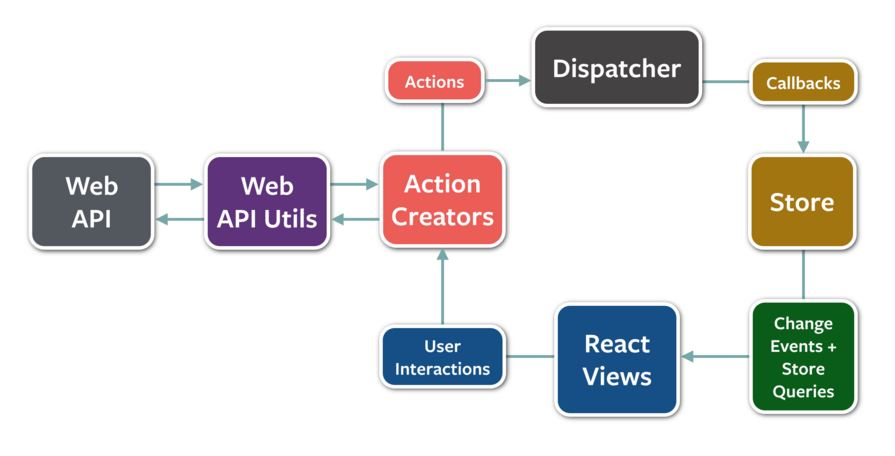
\includegraphics[width=0.8\textwidth]{res/sections/imgs/flux.jpg}
\caption{Diagramma dell'architettura Flux di Facebook}
\end{figure}
In una architettura Flux vengono distinti 4 componenti fondamentali:

\begin{itemize}
\item Action: Rappresenta un messaggio tra le componenti
\item Dispatcher: funge da hub centrale per le action e si occupa di distribuirle al giusto store
\item Store: contengono la logica applicativa del frontend e lo stato dei dati dall'ultimo update. Si occupano di fornire i dati alle viste, quando queste li richiedono
\item View: Sono la parte visiva dell'applicazione e, nel nostro caso, saranno costituite da classi di React.
\end{itemize}

Dall'architettura sopra descritta sono stati individuati i seguenti package per il lato frontend di MaaS:

\begin{figure}[h]
\centering
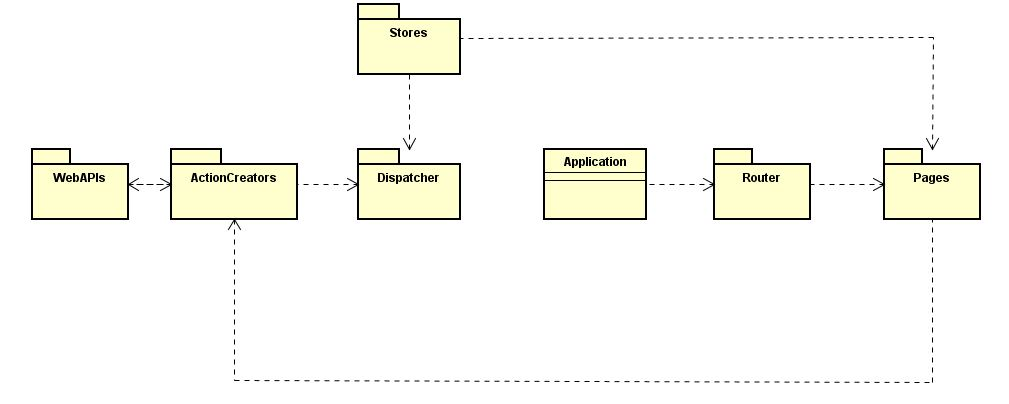
\includegraphics[width=0.8\textwidth]{res/sections/imgs/packages-diagram.jpg}
\caption{Diagramma dei package del frontend}
\end{figure}

\section{Descrizione dei package del frontend}
\subsection{WebAPIs}

\begin{figure}[h]
\centering
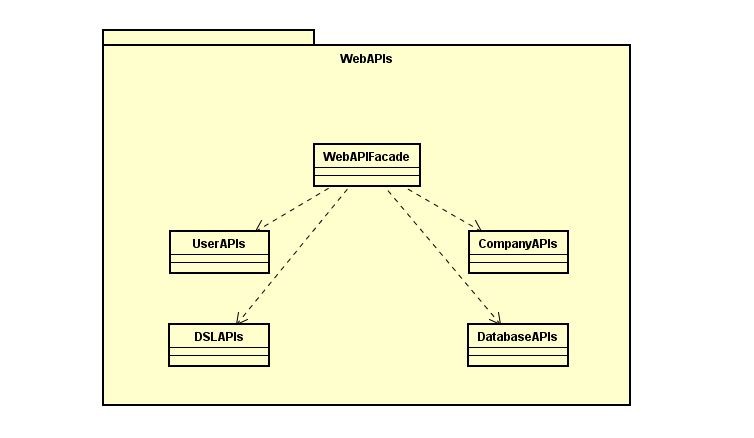
\includegraphics[width=0.8\textwidth]{res/sections/imgs/webapi-diagram.jpg}
\caption{Diagramma dei package del frontend}
\end{figure}

\paragraph*{Descrizione del package}
Il seguente package contiene tutte le classi che contengono i metodi per interagire con le API esposte dal server. 
\paragraph*{Classi contenute}
\begin{itemize}
\item UserAPIs
\item CompanyAPIs
\item DSLAPIs
\item DatabaseAPIs
\item WebAPIFacade
\end{itemize}

\subsubsection{UserAPIs}
\paragraph*{Descrizione della classe}
Classe che espone tutti i metodi per interagire con le API del server che riguardano gli utenti.

\paragraph*{Utilizzo}
Viene utilizzata sia per il login che per gestire le operazioni CRUD per le informazioni riguardanti gli utenti.

\paragraph*{Relazione con altre classi}
\begin{itemize}
\item ActionCreators::UserActionCreator
\end{itemize}

\subsubsection{CompanyAPIs}
\paragraph*{Descrizione della classe}
Classe che espone i metodi per interagire con le API esposte dal server che riguardano le Company.

\paragraph*{Utilizzo}
Contiene le operazioni CRUD per interagire con le informazioni riguardanti le company utilizzando le API esposte dal backend.

\paragraph*{Relazione con altre classi}
\begin{itemize}
\item ActionCreators::CompanyActionCreator
\end{itemize}

\subsubsection{DSLAPIs}
\paragraph*{Descrizione della classe}
Classe che espone i metodi per interagire con le API esposte dal server che riguardano le specifiche DSL.

\paragraph*{Utilizzo}
Viene utilizzata per lanciare le operazioni CRUD associate alle API esposte dal backend.

\paragraph*{Relazione con altre classi}
\begin{itemize}
\item ActionCreators::DSLActionCreator
\end{itemize}

\subsubsection{DatabaseAPIs}
\paragraph*{Descrizione della classe}
Classe per interagire con le API esposte dal server che riguardano i Database delle company.

\paragraph*{Utilizzo}
Viene utilizzata questa classe per lanciare le operazioni CRUD esposte dalle API del backend.

\paragraph*{Relazione con altre classi}
\begin{itemize}
\item ActionCreators::DatabaseAPIs
\end{itemize}

%% FACADE?

\subsection{ActionCreators}

\begin{figure}[h]
\centering
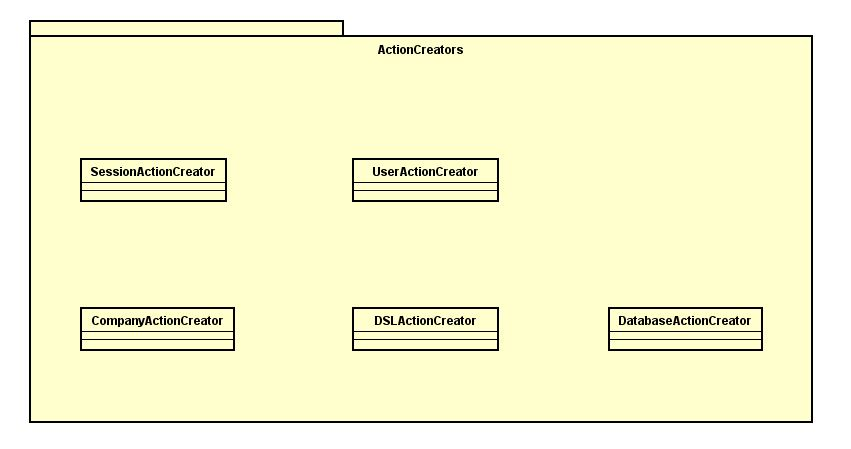
\includegraphics[width=0.8\textwidth]{res/sections/imgs/actioncreator-diagram.jpg}
\caption{Diagramma dei package del frontend}
\end{figure}


\paragraph*{Descrizione del package}
Questo package contiene tutte le classi che si prestano come factory di Action. Le classi in questione mettono in relazione le webAPIs con il resto dell'applicazione, cioè vengono utilizzate per la richiesta delle funzionalità delle webAPIs per poi lanciare le Action relative alle risposte ricevute.

\paragraph*{Classi contenute}
\begin{itemize}
\item SessionActionCreator
\item UserActionCreator
\item CompanyActionCreator
\item DSLActionCreator
\item DatabaseActionCreator
\end{itemize}

\subsubsection{SessionActionCreator}
\paragraph*{Descrizione della classe}
Classe che si occupa della gestione delle action relative alla sessione corrente.

\paragraph*{Utilizzo}
Viene utilizzata per richiedere il login di un utente e per emanare le action relative a login, sessione corrente e logout.

\paragraph*{Relazione con altre classi}
\begin{itemize}
\item Dispatcher
\item (Stores::SessionStore)
\item Pages::LoginPage
\end{itemize}

\subsubsection{UserActionCreator}
\paragraph*{Descrizione della classe}
Classe che si occupa di creare e lanciare le action relative agli utenti.
\paragraph*{Utilizzo}
Viene utilizzata per creare le action relative agli utenti: la classe fornisce i metodi per utilizzare le webAPIs contenute in UserAPIs e restituisce le action che poi verrano reindirizzate a UserStore.

\paragraph*{Relazione con altre classi}
\begin{itemize}
\item Dispatcher
\item (Stores::UserStore)
\item Pages::ProfilePage
\item Pages::ModifyProfilePage
 %% ...
\end{itemize}

\subsubsection{CompanyActionCreator}
\paragraph*{Descrizione della classe}
Classe che si occupa dell'interazione dell'applicazione con CompanyAPIs e di lanciare Action relative alle risposte ottenute da essa.
\paragraph*{Utilizzo}
La classe viene utilizzata per creare le action relative alle Company: sfrutta i metodi dichiarati in CompanyAPIs per interagire con il server e lancia le action contenenti i dati ricevuti dalle API richieste.

\paragraph*{Relazione con altre classi}
\begin{itemize}
\item Dispatcher
\item (Stores::CompanyStore)
\item Pages::CompanyPage
%% ...
\end{itemize}

\subsubsection{DSLActionCreator}
\paragraph*{Descrizione della classe}
Classe che si occupa di creare action riguardanti le specifiche DSL.
\paragraph*{Utilizzo}
Tale classe viene utilizzata per sfruttare i metodi dichiarati in DSLAPIs per la richiesta delle API esposte dal server relative alle specifiche DSL. Dopo aver sfruttato l'API richiesta, la classe crea un'action contenente i risultati ottenuti.

\paragraph*{Relazione con altre classi}
\begin{itemize}
\item Dispatcher
\item (Stores::DSLStore)
\item DSLPage
\end{itemize}

\subsubsection{DatabaseActionCreator}
\paragraph*{Descrizione della classe}
Classe che si occupa di lanciare action riguardanti le connessioni ai Database di una Company.
\paragraph*{Utilizzo}
La classe viene utilizzata per richiamare i metodi definiti in DatabaseAPIs e creare le action contenenti le risposte dai metodi chiamati.
\paragraph*{Relazione con altre classi}
\begin{itemize}
\item Dispatcher
\item (Store::DatabaseStore)
\item Pages::DatabaseCollectionPage
\item Pages::SingelDatabasePage
\item Pages::CreateDatabasePage
\item Pages::ModifyDatabasePage
\end{itemize}

\subsection{Dispatcher}
\paragraph*{Descizione della classe}
Classe raffigurante il dispatcher descritto nell'architettura Flux.
\paragraph*{Utilizzo}
Il dispatcher viene utilizzato come hub centrale delle action circolanti per l'applicazione. Con esso viene definito il punto di destinazione delle action prodotte dai creators.
\paragraph*{Relazione con altre classi}
\begin{itemize}
\item Stores
\item ActionCreators
\end{itemize}


\subsection{Stores}

\begin{figure}[h]
\centering
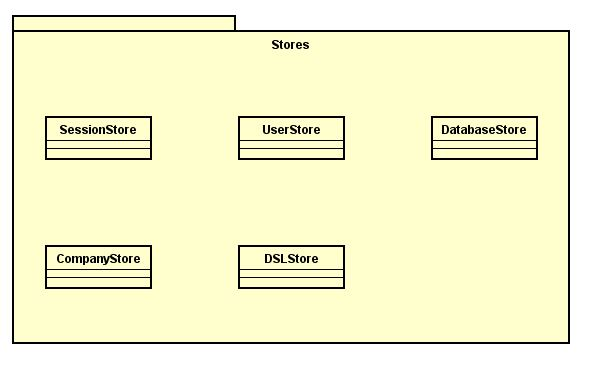
\includegraphics[width=0.8\textwidth]{res/sections/imgs/stores-diagram.jpg}
\caption{Diagramma di deployment per l'architettura}
\end{figure}

\paragraph*{Descrizione del package}
Il package in questione contiene le classi che implementano il concetto di Store presentato nell'architettura Flux. Ciascuno Store contiene dei dati omogenei tra loro e si occupa di fornirli alle pagine che ne necessitano.
\paragraph*{Classi contenute}
\begin{itemize}
\item SessionStore
\item UserStore
\item DatabaseStore
\item CompanyStore
\item DSLStore
\end{itemize}

\subsubsection{SessionStore}
\paragraph*{Descrizione della classe}
Classe che contiene i dati relativi alla sessione corrente.
\paragraph*{Utilizzo}
Classe che viene utilizzata dall'applicazione per contenere e fornire i dati relativi alla sessione corrente. Si occupa di gestire le action relative alla sessione e di conservarne i dati.
\paragraph*{Relazione con altre classi}
\begin{itemize}
\item Router
\item Pages
\end{itemize}

\subsubsection{UserStore}
\paragraph*{Descrizione della classe}
Classe che si occupa di contenere i dati relativi agli User.
\paragraph*{Utilizzo}
Questa classe viene utilizzata per mantenere i dati riguardanti gli utenti e di fornirli alle pagine che li richiedono.
\paragraph*{Relazione con altre classi}
\begin{itemize}
\item Pages
\item Dispatcher
\end{itemize}

\subsubsection{DatabaseStore}
\paragraph*{Descrizione della classe}
Classe che si occupa di contenere i dati relativi alle connessioni ai database definiti per le Company.
\paragraph*{Utilizzo}
Questa classe viene utilizzata per contenere i dati riguardanti le connessioni dei database definiti per le company. Si occupa di ricevere dal dispatcher le action relative a questi dati e di mantenere i dati riferiti.
\paragraph*{Relazione con altre classi}
\begin{itemize}
\item Pages
\item Dispatcher
\end{itemize}

\subsubsection{CompanyStore}
\paragraph*{Descrizione della classe}
Classe che si occupa di contenere i dati relativi alle Company.
\paragraph*{Utilizzo}
Questa classe viene utilizzata per ricevere le action relative alle Company al fine di mantenere i dati relativi ad esse. Inoltre fornisce i metodi per fornire tali dati alle pagine che li richiedono
\paragraph*{Relazione con altre classi}
\begin{itemize}
\item Dispatcher
\item Pages
\end{itemize}

\subsubsection{DSLStore}
\paragraph*{Descrizione della classe}
Classe che si occupa di contenere i dati delle specifiche DSL
\paragraph*{Utilizzo}
Questa classe fornisce i metodi per ricevere le Action relative alle specifiche DSL e per mantenere i dati relativi ad esse. Fornisce inoltre i metodi per disporre quei dati per le pagine che li richiedono.
\paragraph*{Relazione con altre classi}
\begin{itemize}
\item Dispatcher
\item Pages
\end{itemize}


\subsection{Application}
\paragraph*{Descrizione della classe}
Questa è la classe principale del frontend: è la classe che richiama il router e che inizializza il frontend.
\paragraph*{Utilizzo}
Viene utilizzata per inizializzare il frontend e per fornire le configurazioni necessarie al funzionamento per l'applicazione.

\subsection{Router}
\paragraph*{Descrizione della classe}
Questa classe è necessaria all'applicazione per determinare quale pagina mostrare.
\paragraph*{Utilizzo}
Viene istanziata in nell'applicazione principale e determina le associazioni tra pagine e URL per identificarle.

\subsection{Pages}
\paragraph*{Descrizione del package}
Questo package contiene tutte le pagine richiamate da Router. Ciascuna classe rappresenta una pagina definita come componente React e fornisce i metodi alla pagina per recuperare i dati da mostrare dagli store e i metodi per richiamare gli ActionCreators per la creazione di nuove Action.
